\documentclass[10pt,a4paper,landscape]{article}
\usepackage[T1]{fontenc}\usepackage[utf8]{inputenc}\usepackage[spanish]{babel}
\usepackage{lmodern,geometry,booktabs,longtable,graphicx,hyperref}
\geometry{margin=1.7cm}\setlength{\parindent}{0pt}\setlength{\parskip}{6pt}
\setlength{\emergencystretch}{3em}
\begin{document}
\begin{center}{\LARGE Proyecto 4 -- Testbench de todas las acciones}\\[5pt]
Cristian Acevedo -- Guillermo Arriaza -- Eduardo Ponce\end{center}
\textbf{Alcance.} Se simula Espino RV32E, el firmware de tendencia lenta y el
SPI activo; cada escenario comienza con caja de \$10\,000, cero acciones y
comisión de \$5 por orden ejecutada. Se comprueban MISO, DECISION, caja,
inventario, fills, comisiones y patrimonio por tick, secuencia MMIO, SUM10,
recepción única, registros internos, reinicio y plazo de respuesta.

\textbf{Placa real.} El usuario informó haber reprogramado la FPGA. Este ensayo
no lee la flash ni recibe telemetría de la placa; no certifica su cableado ni
el resultado de la competencia física. Verilator simula en dos estados y
complementa las pruebas previas de cuatro estados con Icarus.

\textbf{Datos.} Ocho series de práctica y 35 CSV adicionales del ZIP, cada uno
en dos escalas: proporcional y afín. Las escalas no son muestras independientes.
Se usan hasta 20\,000 ticks: GOOGL 2021 contiene 18\,844 y Disney 2022,
19\,966. Se prueban sin rellenar precios. Las filas sobrantes de otros archivos
quedan fuera de la ronda. La procedencia externa de los adicionales no se
verificó; su normalización utiliza extremos de la muestra completa como
preprocesamiento retrospectivo y no acredita una transformación causal en vivo.

\textbf{Resultado técnico.} 78/78 PASS; 1,557,620 ticks; cero discrepancias. Cadencia: 100 microsegundos. Peor tiempo observado: 20.72 microsegundos.

\textbf{Resultado financiero.} PASS indica equivalencia técnica, no ganancia.
No operar conserva \$10\,000. Mantener es el benchmark ideal del curso, con
una comisión inicial y sin límite de 63. La estrategia empieza en caja, revisa
SUM10 cada 128 ticks y cambia de régimen con 5\%; puede no operar.

\begin{center}\begin{tabular}{lrrrrrrr}\toprule
Grupo & Casos & PASS & Supera mantener & Sin órdenes & Patrimonio medio & Peor & DD máx. (\%) \\\midrule
Ocho conocidas & 8 & 8 & 5 & 0 & 10971.12 & 8540 & 50.55 \\
ZIP proporcional & 35 & 35 & 16 & 15 & 10784.00 & 5863 & 45.34 \\
ZIP afin & 35 & 35 & 18 & 0 & 12150.57 & 5518 & 52.05 \\
\bottomrule\end{tabular}\end{center}
\textbf{Trazabilidad.} BIN SHA-256: \texttt{1f514301f1a7300351f4d3d8f48b77c2c85dcd2a274f44910d11d00df406db45}.
\path{resumen.json} conserva hashes de fuentes, ZIP y trazas. Los CSV por tick,
operaciones, vectores y logs están en \path{build/testbench_todas_acciones/}.
\clearpage\begin{center}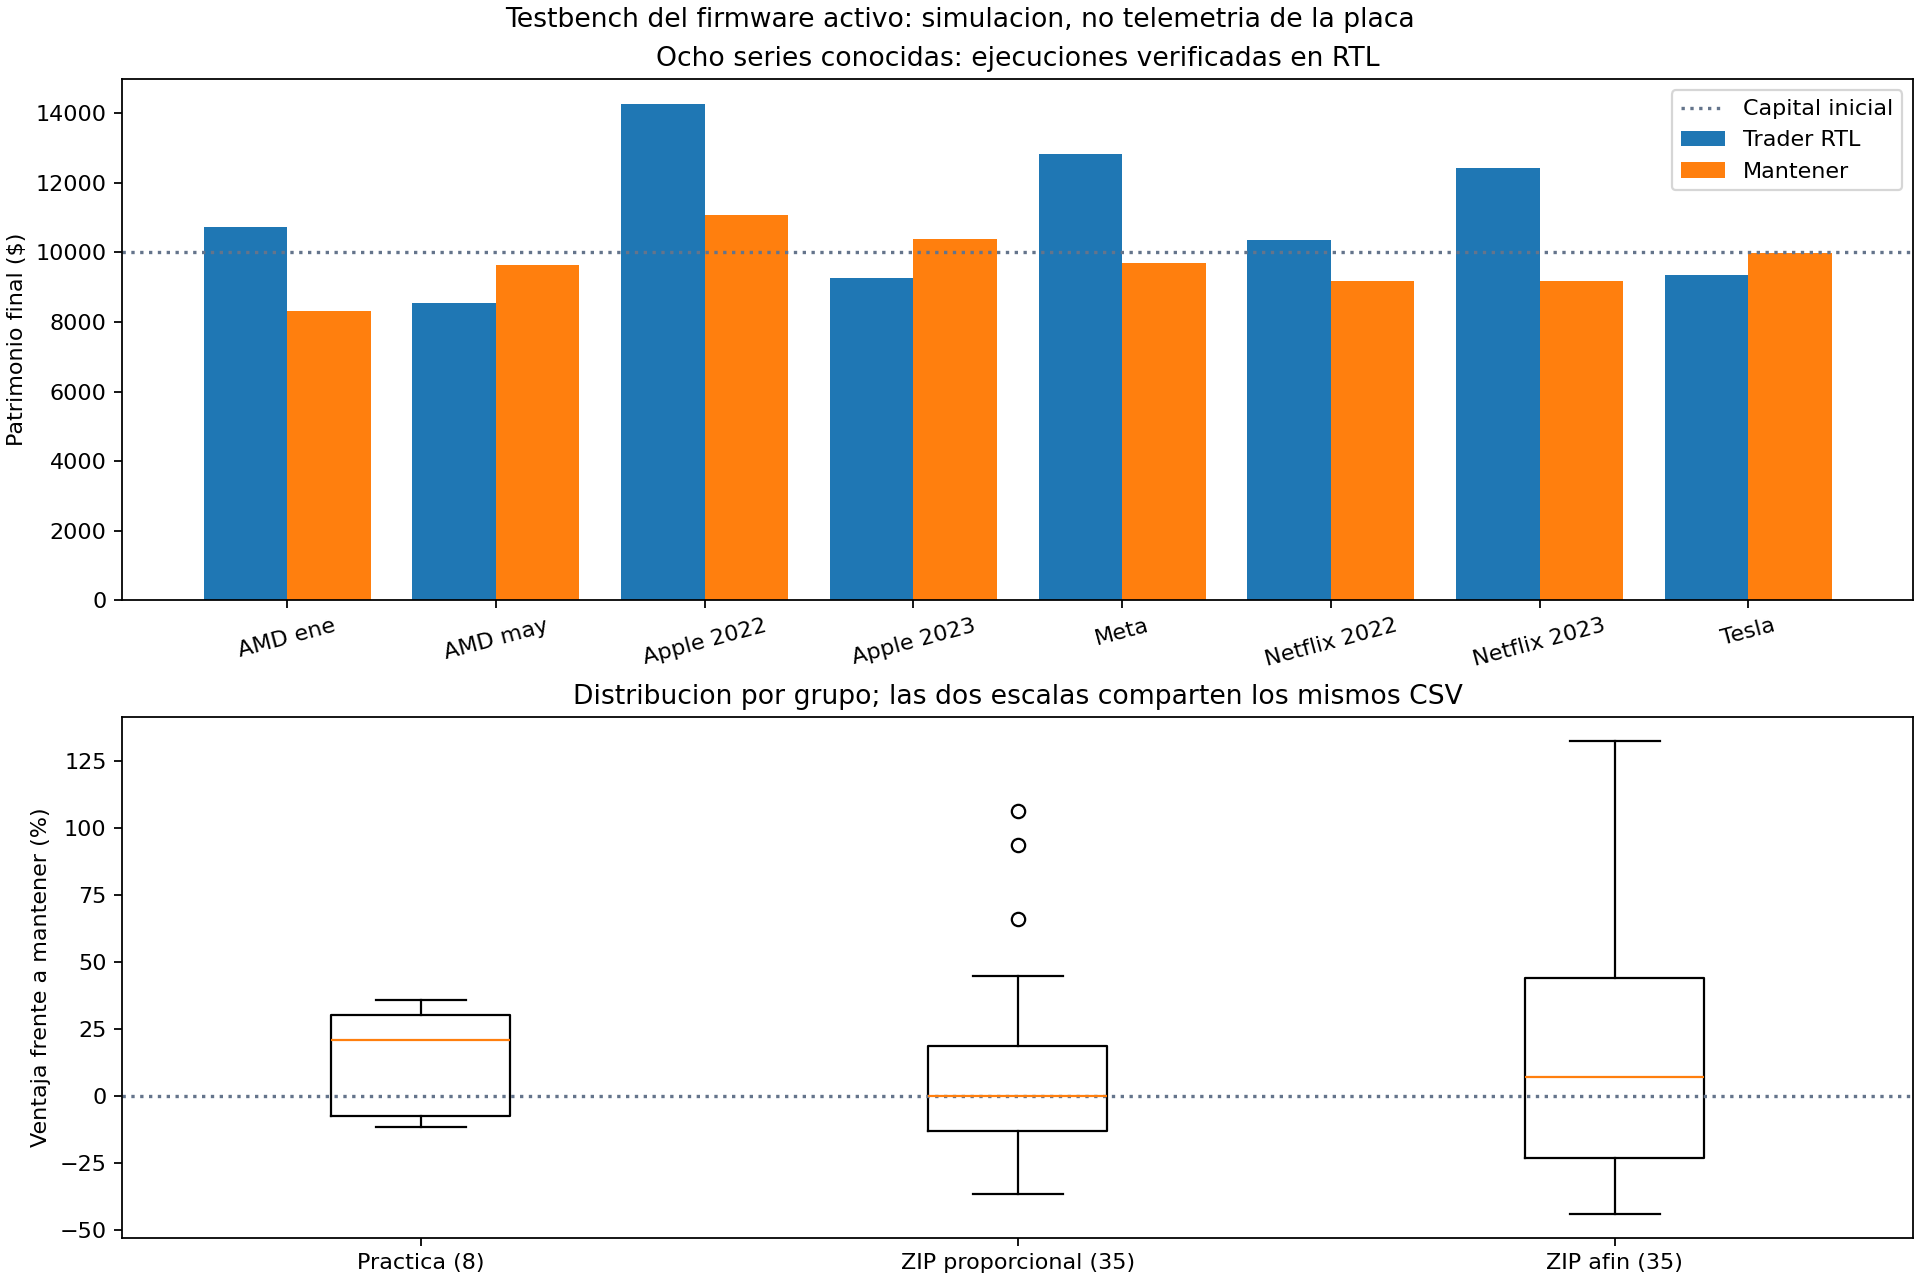
\includegraphics[height=0.9\textheight,keepaspectratio]{grafico_resumen.png}\end{center}
\clearpage\section*{Resultados por escenario}
Los ticks comienzan en cero. Primera compra es el tick de ejecución, no el
de señal; $-1$ indica que no hubo compra en todo el escenario.
\begin{longtable}{lrrrrrrrr}\toprule
Serie y escala & Ticks & Trader & Mantener & Compras & Ventas & DD (\%) & Primera compra & Máx. ($\mu$s) \\\midrule\endhead
practica\_amd\_2022\_ene & 20000 & 10738 & 8315 & 14 & 13 & 42.20 & 257 & 19.92 \\
practica\_amd\_2022\_may & 20000 & 8540 & 9647 & 9 & 8 & 30.01 & 385 & 18.80 \\
practica\_apple\_2022 & 20000 & 14263 & 11063 & 19 & 19 & 38.82 & 385 & 20.72 \\
practica\_apple\_2023 & 20000 & 9272 & 10371 & 14 & 12 & 40.41 & 513 & 20.08 \\
practica\_meta\_2022 & 20000 & 12836 & 9695 & 5 & 5 & 28.13 & 385 & 19.20 \\
practica\_netflix\_2022 & 20000 & 10346 & 9179 & 15 & 15 & 46.72 & 257 & 20.24 \\
practica\_netflix\_2023 & 20000 & 12432 & 9170 & 14 & 12 & 50.55 & 2177 & 19.76 \\
practica\_tesla\_2022 & 20000 & 9342 & 9995 & 8 & 8 & 48.52 & 257 & 17.84 \\
AAPL\_2019-01-02\_afin & 20000 & 16261 & 17585 & 5 & 4 & 18.04 & 897 & 19.92 \\
AAPL\_2020-03-23\_afin & 20000 & 14403 & 21385 & 4 & 4 & 15.14 & 257 & 19.76 \\
AAPL\_2021-01-04\_afin & 20000 & 7578 & 6927 & 16 & 16 & 46.77 & 1281 & 20.24 \\
AAPL\_2022-01-03\_afin & 20000 & 9256 & 5996 & 11 & 10 & 37.84 & 2561 & 19.44 \\
AAPL\_2023-08-01\_afin & 20000 & 12053 & 7070 & 8 & 7 & 31.15 & 6273 & 20.08 \\
AMD\_2022-01-03\_afin & 20000 & 13517 & 5813 & 16 & 14 & 31.98 & 2305 & 20.24 \\
AMD\_2023-05-01\_afin & 20000 & 17992 & 16540 & 6 & 4 & 31.94 & 1281 & 20.40 \\
AMZN\_2020-03-02\_afin & 20000 & 15032 & 15407 & 5 & 5 & 22.36 & 3585 & 19.76 \\
AMZN\_2023-01-03\_afin & 20000 & 18189 & 15058 & 10 & 8 & 18.52 & 1409 & 20.40 \\
BA\_2020-02-03\_afin & 20000 & 11433 & 5417 & 4 & 4 & 14.46 & 11905 & 19.52 \\
DIS\_2022-01-03\_afin & 19966 & 11903 & 6803 & 8 & 6 & 41.75 & 5249 & 19.68 \\
GOOGL\_2021-06-01\_afin & 18844 & 14609 & 21470 & 8 & 7 & 27.80 & 897 & 19.92 \\
GOOGL\_2023-01-03\_afin & 20000 & 9234 & 15995 & 11 & 10 & 45.19 & 1537 & 20.16 \\
INTC\_2022-06-01\_afin & 20000 & 6589 & 4925 & 8 & 7 & 49.20 & 3969 & 19.04 \\
JPM\_2021-01-04\_afin & 20000 & 20698 & 21949 & 7 & 5 & 18.37 & 897 & 20.08 \\
JPM\_2022-01-03\_afin & 20000 & 7387 & 6361 & 9 & 8 & 44.05 & 513 & 18.16 \\
KO\_2019-01-02\_afin & 20000 & 6756 & 7658 & 6 & 5 & 48.62 & 1665 & 18.24 \\
KO\_2022-06-01\_afin & 20000 & 7834 & 10670 & 16 & 16 & 50.24 & 385 & 19.92 \\
META\_2021-03-01\_afin & 20000 & 9564 & 17129 & 10 & 10 & 34.82 & 385 & 20.08 \\
META\_2022-01-03\_afin & 20000 & 5654 & 4847 & 4 & 3 & 52.05 & 5761 & 17.52 \\
META\_2022-11-28\_afin & 20000 & 16031 & 21015 & 6 & 4 & 22.53 & 1153 & 20.24 \\
META\_2023-06-01\_afin & 20000 & 11872 & 16718 & 8 & 7 & 25.65 & 257 & 19.84 \\
MSFT\_2020-02-03\_afin & 20000 & 13587 & 10534 & 11 & 10 & 40.26 & 513 & 20.08 \\
MSFT\_2022-01-03\_afin & 20000 & 10550 & 5900 & 11 & 9 & 26.83 & 4353 & 19.84 \\
MSFT\_2023-01-03\_afin & 20000 & 13756 & 15755 & 10 & 9 & 24.76 & 1537 & 20.40 \\
NFLX\_2022-01-03\_afin & 20000 & 8535 & 4691 & 5 & 3 & 36.27 & 5249 & 19.44 \\
NFLX\_2022-04-01\_afin & 20000 & 5518 & 4583 & 4 & 3 & 48.40 & 513 & 17.20 \\
NVDA\_2022-01-03\_afin & 20000 & 12621 & 6469 & 18 & 16 & 31.17 & 2305 & 20.08 \\
NVDA\_2022-09-01\_afin & 20000 & 8851 & 12645 & 11 & 10 & 42.03 & 385 & 19.12 \\
NVDA\_2023-01-03\_afin & 20000 & 16953 & 22826 & 3 & 2 & 16.67 & 1665 & 19.52 \\
NVDA\_2024-01-02\_afin & 20000 & 16669 & 21557 & 6 & 4 & 16.34 & 1665 & 19.76 \\
TSLA\_2020-06-01\_afin & 20000 & 19510 & 20383 & 6 & 4 & 24.00 & 2049 & 20.24 \\
TSLA\_2021-01-04\_afin & 20000 & 9665 & 9043 & 6 & 6 & 45.73 & 897 & 18.72 \\
TSLA\_2022-01-03\_afin & 20000 & 9905 & 6089 & 6 & 5 & 33.26 & 5761 & 19.44 \\
TSLA\_2023-01-03\_afin & 20000 & 15305 & 16967 & 5 & 5 & 18.37 & 513 & 20.00 \\
AAPL\_2019-01-02\_prop & 20000 & 10000 & 12063 & 0 & 0 & 0.00 & -1 & 5.92 \\
AAPL\_2020-03-23\_prop & 20000 & 13440 & 14307 & 1 & 0 & 9.73 & 513 & 17.60 \\
AAPL\_2021-01-04\_prop & 20000 & 10000 & 9197 & 0 & 0 & 0.00 & -1 & 5.92 \\
AAPL\_2022-01-03\_prop & 20000 & 10000 & 8915 & 0 & 0 & 0.00 & -1 & 5.92 \\
AAPL\_2023-08-01\_prop & 20000 & 10000 & 9293 & 0 & 0 & 0.00 & -1 & 5.92 \\
AMD\_2022-01-03\_prop & 20000 & 9558 & 7635 & 1 & 1 & 24.33 & 7425 & 17.44 \\
AMD\_2023-05-01\_prop & 20000 & 10259 & 13073 & 1 & 0 & 18.91 & 7041 & 16.64 \\
AMZN\_2020-03-02\_prop & 20000 & 12245 & 12245 & 1 & 0 & 8.53 & 5121 & 16.80 \\
AMZN\_2023-01-03\_prop & 20000 & 10000 & 11503 & 0 & 0 & 0.00 & -1 & 6.00 \\
BA\_2020-02-03\_prop & 20000 & 9003 & 4367 & 14 & 12 & 35.57 & 11009 & 20.24 \\
DIS\_2022-01-03\_prop & 19966 & 8995 & 8995 & 1 & 0 & 18.59 & 10241 & 16.72 \\
GOOGL\_2021-06-01\_prop & 18844 & 10000 & 11570 & 0 & 0 & 0.00 & -1 & 5.92 \\
GOOGL\_2023-01-03\_prop & 20000 & 10000 & 11311 & 0 & 0 & 0.00 & -1 & 5.92 \\
INTC\_2022-06-01\_prop & 20000 & 10000 & 8045 & 0 & 0 & 0.00 & -1 & 6.16 \\
JPM\_2021-01-04\_prop & 20000 & 10000 & 12592 & 0 & 0 & 0.00 & -1 & 5.92 \\
JPM\_2022-01-03\_prop & 20000 & 10000 & 8683 & 0 & 0 & 0.00 & -1 & 5.92 \\
KO\_2019-01-02\_prop & 20000 & 10000 & 9708 & 0 & 0 & 0.00 & -1 & 6.08 \\
KO\_2022-06-01\_prop & 20000 & 10000 & 10115 & 0 & 0 & 0.00 & -1 & 5.92 \\
META\_2021-03-01\_prop & 20000 & 10000 & 11514 & 0 & 0 & 0.00 & -1 & 5.92 \\
META\_2022-01-03\_prop & 20000 & 10184 & 6134 & 1 & 0 & 3.13 & 19585 & 18.80 \\
META\_2022-11-28\_prop & 20000 & 14322 & 15929 & 2 & 1 & 13.71 & 1153 & 18.80 \\
META\_2023-06-01\_prop & 20000 & 9410 & 11264 & 1 & 0 & 8.10 & 14721 & 17.36 \\
MSFT\_2020-02-03\_prop & 20000 & 12035 & 10253 & 1 & 0 & 11.39 & 12545 & 17.12 \\
MSFT\_2022-01-03\_prop & 20000 & 10000 & 8669 & 0 & 0 & 0.00 & -1 & 5.92 \\
MSFT\_2023-01-03\_prop & 20000 & 10000 & 11480 & 0 & 0 & 0.00 & -1 & 5.92 \\
NFLX\_2022-01-03\_prop & 20000 & 11568 & 5978 & 3 & 1 & 13.72 & 5761 & 19.84 \\
NFLX\_2022-04-01\_prop & 20000 & 5863 & 4747 & 3 & 2 & 45.34 & 513 & 17.60 \\
NVDA\_2022-01-03\_prop & 20000 & 11809 & 8155 & 2 & 1 & 11.47 & 5761 & 17.60 \\
NVDA\_2022-09-01\_prop & 20000 & 10793 & 11271 & 1 & 0 & 2.69 & 19201 & 16.88 \\
NVDA\_2023-01-03\_prop & 20000 & 16043 & 17447 & 1 & 0 & 11.03 & 1665 & 19.28 \\
NVDA\_2024-01-02\_prop & 20000 & 11387 & 18003 & 1 & 0 & 12.73 & 13697 & 16.64 \\
TSLA\_2020-06-01\_prop & 20000 & 14385 & 17366 & 3 & 2 & 17.79 & 2817 & 19.60 \\
TSLA\_2021-01-04\_prop & 20000 & 11289 & 9456 & 2 & 1 & 15.96 & 1281 & 17.44 \\
TSLA\_2022-01-03\_prop & 20000 & 9885 & 7412 & 1 & 0 & 24.41 & 7169 & 17.52 \\
TSLA\_2023-01-03\_prop & 20000 & 14967 & 15251 & 1 & 1 & 13.35 & 1665 & 19.52 \\
\bottomrule\end{longtable}
\end{document}
